% !TEX root = Pflichtenheft.tex


\documentclass[11pt, a4paper, oneside]{memoir}                                                      %%
\usepackage[utf8]{inputenc}
\usepackage[ngerman]{babel}     % new german spelling, umlauts and other regional settings like date format
\usepackage[shortlabels]{enumitem}
\usepackage{nameref,zref-xr}
\zxrsetup{toltxlabel}
\usepackage{graphicx}           % allow for inclusion of images
\usepackage[table,svgnames]{xcolor} % define colors
\usepackage{url}                % weblinks, etc.
\usepackage{colortbl}           % colored table cells
\usepackage{longtable}          % tables, which are longer than one page
\usepackage{hyperref}
\usepackage[intlimits]{mathtools}
\hypersetup{
	bookmarksopen=true,                       % expand bookmark tree in acrobat by default
	pdftitle={SEPMP},                         % set title in meta pdf information
	pdfauthor={Teilnehmer 1, Teilnehmer 2, Teilnehmer 3},                             % set author in meta pdf information
	pdfsubject={},                            % set subject in meta pdf information
	pdfkeywords={},                           % set keyword list in meta pdf information
	colorlinks=true,                          % use colored links instead of black ones
	linkcolor=blue,                           % color for internal links
	anchorcolor=black,                        % color for anchor links
	citecolor=black,                          % color for bibliography links
	filecolor=magenta,                        % color for system local links
	urlcolor=blue,                            % color for url links
	plainpages=false,                         % must be false, so that PDF bookmarks work properly
	hypertexnames=false,                      % use guessable names for links; used for correct bookmarks
	linktocpage                               % link page numbers in toc instead of section names
}

\makeatletter
\def\namedlabel#1#2{\begingroup
    #2%
    \def\@currentlabel{#2}%
    \phantomsection\label{#1}\endgroup
}
\makeatother

\newenvironment{lhp}[3]%
{%
	\item [\namedlabel{#3}{/#2\arabic{#1}/}]% \hfill%
	\addtocounter{#1}{10}%
	\begin{description}[leftmargin=0cm, style=sameline]%
}%
{%
	\end{description}%
}

\newenvironment{php}[4]%
{%
	\item [\namedlabel{#4}{/#2\arabic{#1}/} (\ref{#3})] \hfill%
	\addtocounter{#1}{10}%
	\begin{description}[style=sameline]%
}%
{%
	\end{description}%
}

\zexternaldocument*{Lastenheft}

\makeatletter
	\newcommand{\mysubject}{Pflichtenheft}
	\newcommand{\mygroup}{Gruppe 7}
	\newcommand{\myauthor}{%
		Yonjgun Kim\\
		Ilias Eksi\\
		Tianni Rwema\\
		Leyla Munyana \\
		Cyusa Lucas \\ 
	}
\makeatother

\begin{document}

	\thispagestyle{empty}
	\newcommand{\Rule}{\rule{\textwidth}{0.5mm}}
	\begin{center}
	% upper part
	{\Large 
\includegraphics[height=40mm]{img/RPTU_LOGO_SCHWARZ} \par}

	\vspace{3em}

	{\Large AG Human Computer Interaction \\ apl. Prof. Dr. Achim Ebert \par}

	\vspace{0.5em}

	{\Large SEP \the\year \par}


	\vspace{2cm}

	% middle part
	\Rule

	\vspace{1cm}

	{\Huge Cosmic Eidex \par}

	\vspace{0.5em}

	{\Large \mysubject \par}

	\vspace{0.5em}

	{\small \today \par}

	\vspace{0.7cm}

	\Rule


	\vfill %%%%%%%%%%%%%%%%%%%%%%%%%%%%%%%%%%%%%%%%%%%%%%%%%%%%%%%%%%%%%%%%


	% lower part
	\emph{\textbf{\mygroup}} \\[1em]
	\myauthor

	\end{center}


	\tableofcontents

	\chapter{Projekttreiber}

\section{Vorbemerkung}

Das Lasten- und Pflichtenheft wird als technische Beschreibungen gesehen, entsprechend sind zu besseren Übersichtlichkeit die Vorlagen nicht gegendert. Es bleibt den einzelnen Gruppen vorbehalten, ob sie Dokumente, Dokumentation und GUI gendern oder nicht (fließt entsprechend nicht in die Bewertung mit ein).

\section{Projektziel}

Im Rahmen des Software-Entwicklungs-Projekts {\the\year} soll ein einfach zu bedienendes Client-Server-System zum Spielen von \textit{Cosmic Eidex} über ein Netzwerk implementiert werden. Die Benutzeroberfläche soll intuitiv bedienbar sein.

\section{Stakeholders}

\newcounter{sh}\setcounter{sh}{10}

\begin{description}[leftmargin=5em, style=sameline]
	
	\begin{lhp}{sh}{SH}{sh:Spieler}
		\item [Name:] Spieler
		\item [Beschreibung:] Menschliche Spieler.
		\item [Ziele/Aufgaben:] Das Spiel zu spielen.
	\end{lhp}
	
	\begin{lhp}{sh}{SH}{bsh:Spieler}
		\item [Name:] Eltern
		\item [Beschreibung:] Eltern minderjähriger Spieler.
		\item [Ziele/Aufgaben:] Um die Spieler zu kümmern, indem Eltern Spielzeit begrenzen wollen und zugriff auf sensible Inhalte begrenzen.
	\end{lhp}
	
	\begin{lhp}{sh}{SH}{bsh:gesetzgeber}
		\item [Name:] Gesetzgeber
		\item [Beschreibung:] Das Amt für Jugend und Familie.
		\item [Ziele/Aufgaben:] Die Rechte der Spieler zu schützen und zu gewähren, indem er Gesetze erstellt.
	\end{lhp}
	
	\begin{lhp}{sh}{SH}{bsh:investor}
		\item [Name:] Investoren (nur für Beispielzwecken)
		\item [Beschreibung:] Parteien, die das Finanzmittel für die Entwicklung des Systems bereitstellen.
		\item [Ziele/Aufgaben:] Gewinn zu ermitteln, indem das System an Endverbraucher verkauft wird.
	\end{lhp}
	
	\begin{lhp}{sh}{SH}{bsh:betreuer}
		\item [Name:] Betreuer
		\item [Beschreibung:] HiWis, die SEP Projektgruppen betreuen.
		\item [Ziele/Aufgaben:] Das Entwicklungsprozess zu betreuen, zu überwachen und teilweise zu steuern als auch die Arbeit der Projektgruppen abzunehmen sowie den Studenten im Prozess Hilfe zur Verfügung zu stellen. 
	\end{lhp}
	
	\begin{lhp}{sh}{SH}{bsh:prof}
		\item [Name:] apl. Prof. Dr. Achim Ebert
		\item [Beschreibung:] Der Leiter des gesamten Projekts
		\item [Ziele/Aufgaben:] Die HiWis anleiten, ihnen sagen, worauf sie bei den Projekten achten sollen und ihnen helfen, wenn sie Probleme haben.
	\end{lhp}
		
\end{description}

\section{Aktuelle Lage}

Aktuell wird das Spiel Cosmic Eidex persönlich gespielt, wo die Spieler zusammen in einem Raum sein müssen und die Karten wie bei jedem anderen Kartenspiel ausgeteilt werden und jeder Spieler die Spielregeln kennen sollte. Das Problem ist, dass die Spieler alle im selben Raum sein müssen, um das Spiel zu spielen und wenn das Regelbuch nicht direkt zugänglich ist, muss man darauf vertrauen, dass die anderen Spieler die Regeln auswendig kennen. Das Ziel dieses Projekts ist es, eine digitale Version von Cosmic Eidex zu erstellen, die es den Benutzern ermöglicht, gemeinsam online zu spielen und mit Leuten aus verschiedenen Orten zu interagieren. Der Benutzer kann sich in das Spiel einloggen und Spielräumen beitreten, die in der Lobby sichtbar sind. In diesen Spielräumen können die Spieler dann ein Spiel beginnen, wenn die erforderliche Anzahl von Spielern erreicht ist, um das Spiel zu starten. Sowohl in der Lobby als auch in den Spielräumen können die Spieler über die Chat-Funktion miteinander kommunizieren. Darüber hinaus wird ein Bot-Spieler hinzugefügt, falls der Spieler selbst üben und seine Kenntnisse des Spiels verfeinern möchte. Und die Eltern profitieren davon, dass sie sehen können, wie lange die Kinder spielen und sicher sind, dass sie nicht zu lange spielen. 
	\chapter{Projektbeschränkungen}

\section{Beschränkungen}

\newcounter{lb}\setcounter{lb}{10}

\begin{description}[leftmargin=5em, style=sameline]
	
	\begin{lhp}{lb}{LB}{beschr:lehrbots}
		\item [Name:] Selbstlehrende Bots
		\item [Beschreibung:] Keine Selbstlehrfunktion von Bots wird implementiert.
		\item [Motivation:] Die Funktionalität ist zu aufwändig zu implementieren und passt deshalb nicht in das Zeitbudget.
		\item [Erfüllungskriterium:] Intelligenzalgorithmus von Bots ist so vorprogrammiert, dass sie Entscheidungen nur anhand des vorprogrammierten Wissens sowie des aktuellen Spielstands treffen, ohne dabei frühere Spiele zu berücksichtigen.
	\end{lhp}
	
	\begin{lhp}{lb}{LB}{beschr:anwendungsbereich}
		\item [Name:] Anwendungsbereich
		\item [Beschreibung:] Das System ist ausschließlich für den privaten Bereich ausgelegt.
		\item [Motivation:] Die Wartung ist teuer
		\item [Erfüllungskriterium:] Benutzer- und Spieldaten sollten unsere aktuelle Serverkapazität nicht überschreiten
	\end{lhp}
	
		
	\begin{lhp}{lb}{LB}{beschr:implsprache}
		\item [Name:] Implementierungssprache
		\item [Beschreibung:] Für die Implementierung ist ausschließlich Java 8 oder höher zu verwenden.
		\item [Motivation:] Das optimiert die Betreuung vom SEP und koordiniert die Mitarbeit.
		\item [Erfüllungskriterium:] Es sollte eine Version von Java 8 oder höher verwendet werden
	\end{lhp}
	
	\begin{lhp}{lb}{LB}{beschr:gui}
		\item [Name:] GUI-Framework
		\item [Beschreibung:] Die GUI ist mit JavaFX zu realisieren.
		\item [Motivation:] Das optimiert die Betreuung vom SEP und koordiniert die Mitarbeit.
		\item [Erfüllungskriterium:] Alle GUIs sollten mit JavaFX entwickelt werden
	\end{lhp}
	
	\begin{lhp}{lb}{LB}{beschr:gitlab}
		\item [Name:] Gitlab
		\item [Beschreibung:] Für die Entwicklung ist das vorgegebene GitLab-Repository zu verwenden.
		\item [Motivation:] Das optimiert die Betreuung vom SEP und koordiniert die Mitarbeit.
		\item [Erfüllungskriterium:] Der gesamte Projektcode und die Dokumentation werden zur besseren Beurteilung auf Gitlab hochgeladen
	\end{lhp}
	
	
\end{description}

\section{Glossar}

\begin{center}
		\rowcolors{2}{Gray!15}{White}
		\begin{longtable}{p{0.25\textwidth} p{0.25\textwidth} p{0.4\textwidth}}
			\textbf{Deutsch} & \textbf{Englisch} & \textbf{Bedeutung} \\
			\hline \hline \endhead                      
			Bot & bot & Spieler, dessen Spielaktionen vom Computer entschieden und durchgeführt werden\\
			Kekse & Cookies & Offiziell keine gültige Maßnahme zur Bestechung der HiWis\\          
 			Lobby & lobby & Virtueller Raum zum Betreten eines Spielraums\\	
			Spiel (Regelwerk) & game & Cosmic Eidex \\
			Spieler & player & Teilnehmer am Spielgeschehen\\
			Spielraum & game room & Virtueller Raum, in dem ein Spiel stattfindet\\
			Zug & turn & Zustand in dem ein Spieler eine Spielaktion ausführen muss\\
            Bestenliste & leaderboard & Zeigt den Punktestand aller Spieler an\\
            Karten & cards & Spielkarten, die im Spiel verwendet werden\\
            Trumpf & trump & Die spezielle Kartenfarbe (z. B. Herz), die alle anderen Farben in einem Stich übertrumpft. Die Trumpffarbe wird zu Beginn eines Stichs aufgedeckt, wenn eine Karte abgelegt wird.\\
            Cosmic Charaktere & cosmic characters & Charakter auf der Karte, der dem Spieler besondere Kräfte verleiht, die einmal pro Runde eingesetzt werden \\
            Drücker & buried card & Eine Karte, die nicht gespielt wird und dem Spieler, der sie versteckt hat, Punkte einbringt\\
            Match & match & Ein Spieler, der jeden Stich in der Hand gewinnt \\ 
            Stich & trick & eine Spielrunde\\
            Deck & deck & Satz von 36 Karten(Herz(rot), Eidex(grün), Raben(schwarz), Sterne(gelb))\\
            
		\end{longtable}
\end{center}

\section{Relevante Fakten und Annahmen}

Wichtige bekannte Fakten und getroffene Annahmen, die sich auf das Projekt direkt oder indirekt beziehen und dadruch auf die zukünftige Implementierungsentscheidungen Effekt haben können.

\newcounter{fa}\setcounter{fa}{10}

\begin{description}[leftmargin=5em, style=sameline]
	
	\begin{lhp}{fa}{FA}{fa:fortentwicklung}
		\item [Name:] Keine Fortentwicklung der App nach dem SEP.
		\item [Beschreibung:] Nach Ende des SEP wird das Projekt nicht weiterentwickelt.
		\item [Motivation:] Das Entwicklungsteam hat keine Lust darauf.
	\end{lhp}
	
	\begin{lhp}{fa}{FA}{fa:recht}
		\item [Name:] Keine Lizenzen für Spielartefakte.
		\item [Beschreibung:] Weder die TU Kaiserslautern noch das Spielwerk + die Freizeit GmbH gewahren dem Entwicklungsteam die Rechte für die Spielartefakte.
		\item [Motivation:] Rechtliche Vorsorge.
	\end{lhp}
	
	\begin{lhp}{fa}{FA}{fa:recht-vergangenheit}
		\item [Name:] Keine bekannte Nachteile von Verwendung von Spielartefakten.
		\item [Beschreibung:] Es ist nicht bekannt, dass die SEP-Teilnehmer der letzten Jahre irgendwelche rechtlichen Probleme dadurch gehabt haben, dass sie die Spielartefakten vom Spielwerk + der Freizeit GmbH im Rahmen des SEP eingesetzt haben.
		\item [Motivation:] Rechtliche Vorsorge.
	\end{lhp}
	
	
\end{description}


	\chapter{Funktionale Anforderungen}

%\section{Systemkontext}

\section{Systemfunktionen}

\newcounter{pfc}\setcounter{pfc}{10}

\begin{description}[leftmargin=5em, style=sameline]
	
	\begin{lhp}{pfc}{LF}{funk:spielverw}
		\item [Name:] Spielverwaltung
		\item [Beschreibung:] Das System verwaltet das von mehreren Spielern geteiltes Spiel in einem Spielraum. Das Spiel erfolgt nach den Spielregeln.
	\end{lhp}
    
	\begin{lhp}{pfc}{LF}{funk:regelprüf}
		\item [Name:] Regelprüfung
		\item [Beschreibung:] Das System prüft ob die Regeln in dem angepeiltem Zug eingehalten werden. Dies umfasst die Bedienpflicht, Trumpfregeln, Charakterregeln.
	\end{lhp}

	\begin{lhp}{pfc}{LF}{funk:stichverw}
		\item [Name:] Stichverwaltung
		\item [Beschreibung:] Das System verwaltet die Stiche, es handlet die Karten und wechselt gegebenenfalls den Status.
	\end{lhp}

	\begin{lhp}{pfc}{LF}{funk:chareffdispatch}
		\item [Name:] Character-Effekt-Dispatcher
		\item [Beschreibung:] Das System führt die Charaktereffekte aus.
	\end{lhp}
    
	\begin{lhp}{pfc}{LF}{funk:zugriff}
		\item [Name:] Zugriffsverwaltung
		\item [Beschreibung:] Das System verwaltet den Zugang zum Spiel anhand Benutzerdaten. Spieler können sich registrieren, anmelden, abmelden sowie ihre Kontos löschen.
	\end{lhp}

	\begin{lhp}{pfc}{LF}{funk:spielraum}
		\item [Name:] Verwaltung der Spielräume
		\item [Beschreibung:] Das System verwaltet die Erstellung, Änderung und Löschung der Spielräume.
	\end{lhp}
	
	\begin{lhp}{pfc}{LF}{funk:bestenliste}
		\item [Name:] Bestenliste
		\item [Beschreibung:] Die Anzahl der gewonnen Spiele aller Spieler anzeigen.
	\end{lhp}
	
	\begin{lhp}{pfc}{LF}{funk:bots}
		\item [Name:] Intelligente Bots
		\item [Beschreibung:] Das System verwaltet die Aktionen der Bots mithilfe vordefinierter Entscheidungsalgorithmen und der Bot kann während der Laufzeit nicht selbstständig lernen.
	\end{lhp}
	
	\begin{lhp}{pfc}{LF}{funk:chat}
		\item [Name:] Chat
		\item [Beschreibung:] Spieler können in Echtzeit miteinander interagieren und chatten und auch an einem Spiel teilnehmen.
	\end{lhp}

\end{description}



	\begin{figure}
\centering	
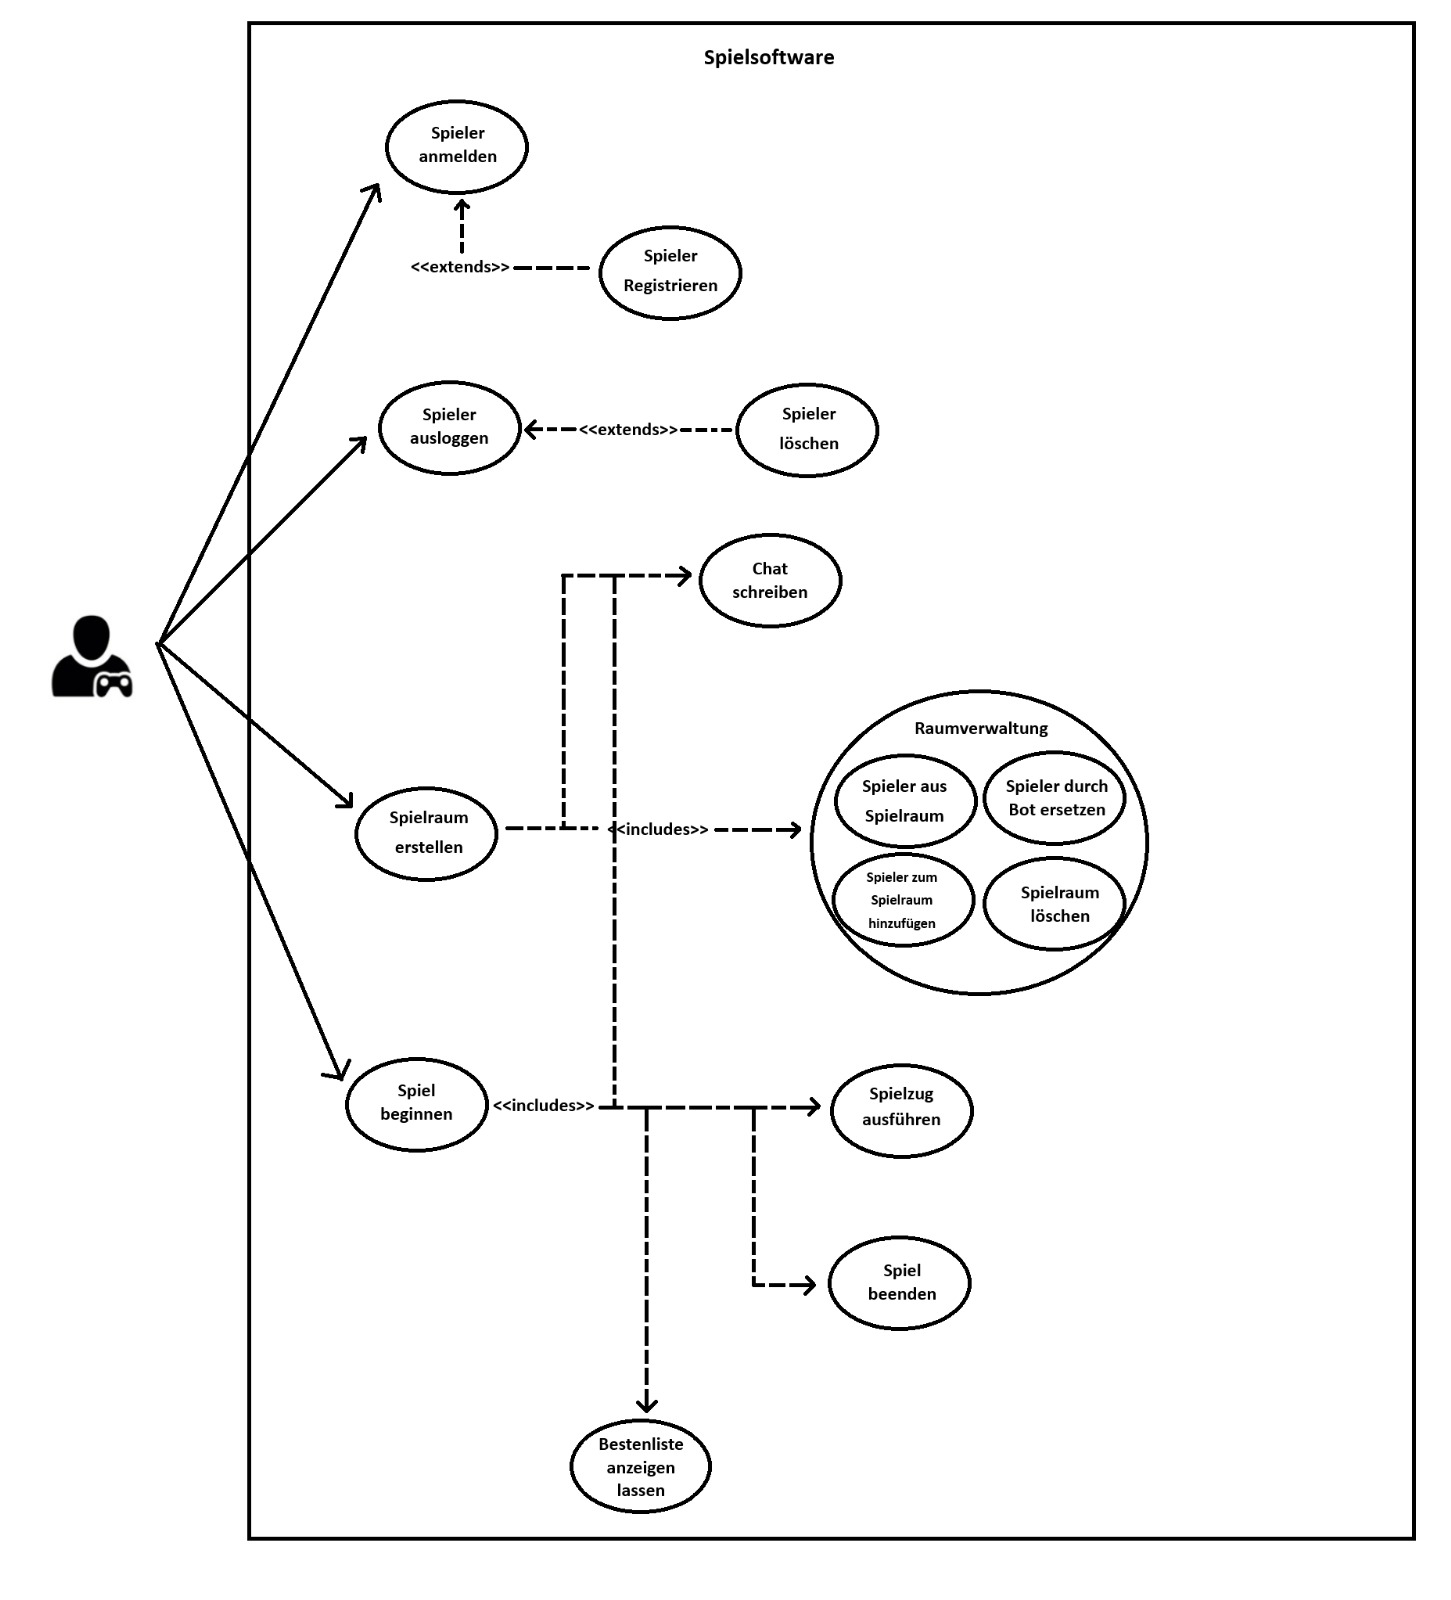
\includegraphics[width=0.9\textwidth]{SEP_Lasten_Pflichtenheft/img/systemedge.jpg}
\label{fig:sys}
\caption{Das Systemgrenzendiagramm}
\end{figure}

\section{Systemgrenze (Use Case Diagramm)}

Die Systemgrenze wird in der Abbildung~\ref{fig:sys} dargestellt


\section{Beschreibungen der Anwendungsfälle}

\newcounter{uc}\setcounter{uc}{10}

\begin{description}[leftmargin=5em, style=sameline]

	\begin{lhp}{uc}{UC}{uc:registrieren}
		\item [Name:] Spieler registrieren.
		\item [Ziel:] Spieler registriert sich im Spiel.
		\item [Akteure:] Spieler.
		\item [Vorbedingungen:] Spieler hat noch keinen Account und befindet sich auf der Login/Registrierungs Seite.
		\item [Eingabedaten:] Zugriffsdaten~\ref{daten:benutzername}Passwort~\ref{daten:passwort}.
		\item [Beschreibung:] Spieler registriert sein Konto.
		\item [Ausnahmen:] Der Benutzername ist bereits vergeben. Das System sendet eine Fehlermeldung.
		\item [Ergebnisse und Outputdaten:] Ein neues Konto wird erstellt. Der Spieler wird angemeldet und in die Lobby versetzt. 
		\item [Systemfunktionen] \ref{funk:zugriff}.
	\end{lhp}
	
	\begin{lhp}{uc}{UC}{uc:anmeld}
		\item [Name:] Spieler anmelden.
		\item [Ziel:] Spieler meldet sich im System an.
		\item [Akteure:] Spieler.
		\item [Vorbedingungen] Spieler ist auf der Registrierungsseite.
		\item [Eingabedaten:] Zugriffsdaten~\ref{daten:benutzername}Passwort~\ref{daten:passwort}.
		\item [Beschreibung:] Spieler meldet sich an.							
		\item [Ausnahmen:] \hfill
			\begin{itemize} 
				\item[] \textit{Passwort oder Benutzername ist falsch:} Das System zeigt eine Fehlermeldung an und der Spieler ist dazu aufgefordert eine erneute Anmeldung zu vollziehen.
				
			\end{itemize}
		\item [Ergebnisse und Outputdaten:] Spieler ist in der Lobby und sieht die Lobby-Seite.
		\item [Systemfunktionen:] \ref{funk:zugriff}.
	\end{lhp}
	
	\begin{lhp}{uc}{UC}{uc:löschen}
		\item [Name:] Spieler löschen.
		\item [Ziel:] Spieler entfernt seine Daten aus dem System.
		\item [Akteure:] Spieler.
		\item [Vorbedingungen] Spieler ist auf der Lobby-Seite.
		\item [Eingabedaten:] Zugriffsdaten~\ref{daten:benutzername}~\ref{daten:passwort}.
		\item [Beschreibung:] Spieler löscht das eigene Konto komplett.
		\item [Ausnahmen:] \hfill
			\begin{itemize} 
				\item[] \textit{Zugriffsdaten sind falsch:} Das System zeigt eine Fehlermeldung an, der Spieler bleibt auf der Seite und kann die Daten erneut eingeben.
			\end{itemize}
		\item [Ergebnisse und Outputdaten:] Spieler wird zur Login-Seite überführt, Spielerkonto wurde gelöscht.	
		\item [Systemfunktionen:] \ref{funk:zugriff}.
	\end{lhp}
    
    \begin{lhp}{uc}{UC}{uc:spielbeginnen}
    \item [Name:] Spiel beginnen.
    \item [Ziel:] Das System startet das Spiel
    \item [Akteure:] System, Spieler
    \item [Vorbedingungen:] Die erforderliche Anzahl an Spielern befindet sich im Spielraum und hat die Ready Checkbox ausgefüllt.
    \item [Eingabedaten:] Benutzername~\ref{daten:benutzername}.
    \item [Beschreibung:] Das Spiel wird gestartet, die Spieler werden zu der Spielbrett-Seite überführt. Das System initialisiert die Spiellogik.
    \item [Ausnahmen:] \hfill
        \begin{itemize}
            \item[] \textit{D:Alle Spieler sind bereit, aber das System startet das Spiel nicht} Das System zeigt eine Fehlermeldung und versucht das Spiel erneut zu starten.
        \end{itemize}
    \item [Ergebnisse und Outputdaten:] Das Spiel beginnt, die Spieler sind auf der Spielbrett-Seite
    \item [Systemfunktionen:] \ref{funk:spielverw}
    \end{lhp}

    \begin{lhp}{uc}{UC}{uc:spielbeenden}
    \item [Name:] Spiel beenden.
    \item [Ziel:] Das System beendet das Spiel, wertet das Ergebnis aus und aktualisiert ggf. Statistiken.
    \item [Akteure:] System
    \item [Vorbedingungen:] Ein Spiel ist derzeit aktiv und ein Spieler oder Bot hat 7 Gewinnpunkte
    \item [Eingabedaten:] Benutzername~\ref{daten:benutzername}, Gewinnpunkte im Spiel~\ref{daten:gw_punkte}, Siege~\ref{daten:siege}.
    \item [Beschreibung:] Das Spiel wird automatisch vom System beendet. Die Ergebnisse werden ausgewertet und gespeichert.
    \item [Ausnahmen:] \hfill
        \begin{itemize}
            \item[] \textit{Kein laufendes Spiel:} Das System zeigt eine Fehlermeldung und versucht zu recovern.
        \end{itemize}
    \item [Ergebnisse und Outputdaten:] Das Spiel ist beendet; Ergebnisse werden gespeichert und ggf. die Bestenliste aktualisiert. Spieler werden in den Spielraum überführt.
    \item [Systemfunktionen:] \ref{funk:spielverw} \ref{funk:bestenliste}
    \end{lhp}

    \begin{lhp}{uc}{UC}{uc:spielerausloggen}
    \item [Name:] Spieler ausloggen.
    \item [Ziel:] Der Spieler meldet sich vom System ab und beendet seine Sitzung.
    \item [Akteure:] Spieler.
    \item [Vorbedingungen:] Der Spieler ist eingeloggt.
    \item [Eingabedaten:] Benutzername~\ref{daten:benutzername}
    \item [Beschreibung:] Der Spieler wählt die Option zur Abmeldung. Das System beendet die Sitzung und schickt den Spieler zum Login-Screen zurück.
    \item [Ausnahmen:] \hfill
        \begin{itemize}
            \item[] \textit{Spieler wurde nicht ausgeloggt:} Das System zeigt eine Fehlermeldung an.
        \end{itemize}
    \item [Ergebnisse und Outputdaten:] Der Spieler ist abgemeldet und der Nutzer befindet sich im Login-Screen.
    \item [Systemfunktionen:] \ref{funk:zugriff}
    \end{lhp}

    \begin{lhp}{uc}{UC}{uc:spielzugausfuehren}
    \item [Name:] Spielzug ausführen.
    \item [Ziel:] Der Spieler führt während seines Spielzugs eine gültige Aktion gemäß den Regeln von Cosmic Eidex aus.
    \item [Akteure:] Spieler, System.
    \item [Vorbedingungen:] Das Spiel läuft (es wurde gestartet und die 36 Karten wurden verteilt) und der Spieler ist am Zug. Die Trumpffarbe steht fest und die vorherigen Stiche wurden abgeschlossen, weiterhin wurden alle Cosmic-Charakter-Effekte verarbeitet.
    \item [Eingabedaten:] Benutzername~\ref{daten:benutzername}, Spielzustand~\ref{daten:gamestate}.
    \item[Beschreibung:]
        \begin{enumerate}
             \item Da der Spieler an der Reihe ist, wird er zur Auswahl einer Karte oder Charakteraktion aufgefordert.
              \item Der Spieler wählt eine Karte aus oder aktiviert einen Charaktereffekt.
              \item Die Gültigkeit des Zuges wird geprüft:
              \begin{enumerate}
                    \item Bedienpflicht oder legaler Trumpf erlaubt.
                    \item Es darf nicht untertrumpft werden, wenn bereits ein Trumpf im Stich liegt.
                   \item Es werden die Cosmic-Charakter-Regeln beachtet.
              \end{enumerate}
              \item Wenn der Zug ungültig ist, wird eine Fehlermeldung gezeigt und Schritt 2 erneut ausgeführt.
              \item Ansonsten wird die Karte zum aktuellen Stich hinzu.
              \item Das System protokolliert den Spielzug
              \item Der folgende Spielverlauf wird geprüft:
                \begin{enumerate}
                    \item Mitspieler müssen noch spielen: Zugrecht wird an nächsten Spieler übergeben und Schritt 1 wird wieder ausgeführt.
                    \item Mitspieler müssen nicht mehr spielen: Stich wird beendet und Stichauswertung wird eingeleitet. ~\ref{uc:stichauswertung}
                \end{enumerate}
        \end{enumerate} 
    \item [Ausnahmen:] \hfill
        \begin{itemize}
            \item[] \textit{Ungültiger Spielzug:} Das System zeigt eine Fehlermeldung und akzeptiert den Zug nicht.
            \item[] \textit{Nicht der Zug des Spielers:} Das System blockiert die Aktion.
            \item[] \textit{Sphinx Effekt:} Karte wird zunächst verdeckt gelegt und erst später aufgedeckt.
            \item[] \textit{Charakterunterbrechung:} Es wird ein spezieller Flow eingeleitet und anschließend bei Schritt 6 weitergemacht.
        \end{itemize}
    \item [Ergebnisse und Outputdaten:] Der Spielzustand wurde entsprechend dem Spielzug aktualisiert. Spielzustand~\ref{daten:gamestate}
    \newline Dies beinhaltet:
    \begin{enumerate}
        \item Aktualisierung der Hand des Spielers
        \item Der Stich erhält eine neue Karte und Auspiel-Metadaten
        \item Das Zugrecht wechselt an den nächsten Spieler oder die Stichauswertung wird eingeleitet
        \item Es werden eventuell ausgelöste Charakter-Events protokolliert
    \end{enumerate}
    \item [Systemfunktionen:] \ref{funk:spielverw} \ref{funk:regelprüf} \ref{funk:stichverw} \ref{funk:chareffdipatch}
    \end{lhp}

    \begin{lhp}{uc}{UC}{uc:chatnachricht}
    \item [Name:] Chat schreiben.
    \item [Ziel:] Der Spieler sendet eine Nachricht im Spielraum-Chat oder Global-Chat.
    \item [Akteure:] Spieler.
    \item [Vorbedingungen:] Der Spieler befindet sich im Spielraum oder in der Lobby oder in der Spielbrett-Seite.
    \item [Eingabedaten:] Benutzername~\ref{daten:benutzername}, Chatnachricht~\ref{daten:msg}
    \item [Beschreibung:] Der Spieler gibt eine Nachricht ein und sendet sie. Das System zeigt sie allen Teilnehmern im Spielraum oder in der Lobby an.
    \item [Ausnahmen:] \hfill
        \begin{itemize}
            \item[] \textit{Leere oder ungültige Nachricht:} Das System versendet die Nachricht nicht.
        \end{itemize}
    \item [Ergebnisse und Outputdaten:] Die Chatnachricht wird allen Spielern im Spielraum oder der Lobby angezeigt.
    \item [Systemfunktionen:] \ref{funk:chat} 
    \end{lhp}

    \begin{lhp}{uc}{UC}{uc:lobbyerstellen}
    \item [Name:] Spielraum erstellen.
    \item [Ziel:] Der Spieler erstellt einen neuen Spielraum, um ein Spiel zu hosten.
    \item [Akteure:] Spieler, System.
    \item [Vorbedingungen:] Der Spieler ist eingeloggt und befindet sich in keinem Spielraum.
    \item [Eingabedaten:] Benutzername~\ref{daten:benutzername}, Spielraumname~\ref{daten:gameroom_name} optional Spielraumpasswort~\ref{daten:gameroom_password}
    \item [Beschreibung:] Der Spieler wählt die Option zum Erstellen einer neuen Lobby. Das System erstellt einen Spielraum und setzt den Spieler als Besitzer ein.
    \item [Ausnahmen:] \hfill
        \begin{itemize}
            \item[] \textit{Name bereits vergeben oder ungültig:} Das System zeigt eine Fehlermeldung und erstellt die Lobby nicht.
        \end{itemize}
    \item [Ergebnisse und Outputdaten:] Ein neuer Spielraum wird erstellt und der Spieler wird als Besitzer eingetragen.
    \item [Systemfunktionen:] \ref{funk:spielraum}
    \end{lhp}
    
    \begin{lhp}{uc}{UC}{uc:lobbyloeschen}
    \item [Name:] Spielraum löschen
    \item [Ziel:] Das System löscht einen Spielraum.
    \item [Akteure:] System
    \item [Vorbedingungen:] Der Spielraum ist leer.
    \item [Eingabedaten:] Spielraumname~\ref{daten:gameroom_name} Spielraumfüllung~\ref{daten:gameroom_pop}.
    \item [Beschreibung:] Das System löscht den Spielraum sobald sich kein Spieler mehr im Raum befindet
    \item [Ausnahmen:] \hfill
        \begin{itemize}
            \item[] \textit{Trotz Spielern wird ein Raum gelöscht:} Das System zeigt eine Fehlermeldung an.
        \end{itemize}
    \item [Ergebnisse und Outputdaten:] Der Spielraum wird gelöscht.
    \item [Systemfunktionen:] \ref{funk:spielraum}
    \end{lhp}
    
    \begin{lhp}{uc}{UC}{uc:spielerlobbyhinzufuegen}
    \item [Name:] Spielraum beitreten
    \item [Ziel:] Ein Spieler tritt einem bestehenden Spielraum bei, um am Spiel teilzunehmen.
    \item [Akteure:] Spieler, System.
    \item [Vorbedingungen:] Der Spielraum existiert und hat einen freien Platz.
    \item [Eingabedaten:] Benutzername~\ref{daten:benutzername}, Spielraumname~\ref{daten:gameroom_name}, Spielraumfüllung~\ref{daten:gameroom_pop} optional Spielraumpasswort~\ref{daten:gameroom_password}.
    \item [Beschreibung:] Der Spieler wählt einen Spielraum aus. Das System fügt den Spieler hinzu, wenn die Bedingungen erfüllt sind.
    \item [Ausnahmen:] \hfill
        \begin{itemize}
            \item[] \textit{Raum ist voll:} Das System zeigt eine Fehlermeldung und lässt keinen Beitritt zu.
            \item[] \textit{Raum nicht gefunden:} Das System zeigt eine Fehlermeldung an.
            \item[] \textit{Falsches Passwort:} Das System zeigt eine Fehlermeldung an.
        \end{itemize}
    \item [Ergebnisse und Outputdaten:] Der Spieler ist dem Spielraum beigetreten und sieht die anderen Teilnehmer.
    \item [Systemfunktionen:] \ref{funk:spielraum}
    \end{lhp}

    \begin{lhp}{uc}{UC}{uc:spielerauslobbyentfernen}
    \item [Name:] Spieler aus Spielraum entfernen.
    \item [Ziel:] Der Besitzer entfernt einen Spieler aus dem aktuellen Spielraum.
    \item [Akteure:] Lobbybesitzer.
    \item [Vorbedingungen:] Der Spielraum existiert und der ausführende Benutzer ist der Besitzer.
    \item [Eingabedaten:] Benutzername~\ref{daten:benutzername}
    \item [Beschreibung:] Der Besitzer wählt einen Spieler aus, der entfernt werden soll. Das System entfernt diesen Spieler aus dem Spielraum.
    \item [Ausnahmen:] \hfill
        \begin{itemize}
            \item[] \textit{Benutzer ist nicht der Besitzer:} Das System verweigert die Aktion.
            \item[] \textit{Spieler konnte nicht entfernt werden:} Das System zeigt eine Fehlermeldung an.
        \end{itemize}
    \item [Ergebnisse und Outputdaten:] Der ausgewählte Spieler wird aus dem Spielraum entfernt und in die Lobby zurückversetzt.
    \item [Systemfunktionen:] \ref{funk:spielraum}
    \end{lhp}

    \begin{lhp}{uc}{UC}{uc:botersetzen}
    \item [Name:] Spieler durch Bot ersetzen.
    \item [Ziel:] Eine freie Stelle im Spielraum wird mit einem Bot aufgefüllt.
    \item [Akteure:] Spielraum-Besitzer, System
    \item [Vorbedingungen:] Es gibt eine freie Stelle im Spielraum oder das Spiel läuft schon und ein Spieler verlässt die Sitzung
    \item [Eingabedaten:] Keine.
    \item [Beschreibung:] Der Besitzer wählt die Option aus einen Bot zum Spielraum hinzuzufügen, das System fügt den Bot hinzu. Falls ein Spieler im Spiel den Gameroom verlässt wird automatisch ein bot hinzugefügt, der das Spiel für den Spieler weiterspielt.
    \item [Ausnahmen:] \hfill
        \begin{itemize}
            \item[] \textit{Keine freie Stelle vorhanden:} Die Option zum auswählen ist nicht anklickbar.
        \end{itemize}
    \item [Ergebnisse und Outputdaten:] Eine Stelle im Spielraum ist nun mit einem Bot besetzt.
    \item [Systemfunktionen:] \ref{funk:spielverw}, \ref{funk:bots}.
    \end{lhp}

    \begin{lhp}{uc}{UC}{uc:bestenlisteanzeigen}
    \item [Name:] Bestenliste anzeigen lassen.
    \item [Ziel:] Der Spieler sieht die Bestenliste mit der Anzahl der gewonnenen Spiele aller Spieler.
    \item [Akteure:] Spieler.
    \item [Vorbedingungen:] Der Spieler befindet sich im Spielraum oder Vorraum.
    \item [Eingabedaten:]
    \item [Beschreibung:] Das System zeigt eine Bestenliste auf Basis der Spielstatistiken an, dies tut es als Teil der GUI.
    \item [Ausnahmen:] \hfill
        \begin{itemize}
            \item[] \textit{Bestenliste nicht verfügbar:} Das System zeigt eine Fehlermeldung anstelle der Bestenliste an
        \end{itemize}
    \item [Ergebnisse und Outputdaten:] Die Bestenliste mit der Anzahl gewonnener Spiele wird angezeigt.
    \item [Systemfunktionen:] \ref{funk:bestenliste}
    \end{lhp}

    \begin{lhp}{uc}{UC}{uc:stichauswertung}
    \item [Name:] Stichauswertung
    \item [Ziel:] Der Stich wird anhand der Spielregeln ausgewertet.
    \item [Akteure:] System
    \item [Vorbedingungen:] Alle Spieler waren am Zug und der Stich muss ausgewertet werden.
    \item [Eingabedaten:] Trumpffarbe ~\ref{daten:trumpf} aktueller Stick ~\ref{daten:stich} 
    \item [Beschreibung:] Das System schaut sich die Stichkarten an und verteilt den Stich an den gewinnenden Spieler.
    \item [Ausnahmen:] \hfill
        \begin{itemize}
            \item[] \textit{System kann auf benötigte Daten nicht zugreifen:} Das System zeigt eine Fehlermeldung an.
        \end{itemize}
    \item [Ergebnisse und Outputdaten:] Der Stich wurde an den gewinnenden Spieler vergeben, und eine neue Spiel/Kartenlegrunde wird initialisiert
    \item [Systemfunktionen:] \ref{funk:bestenliste}
    \end{lhp}
\end{description}
	
\section{Produktdaten}\label{section:productdaten}

Hier sollen die Daten genannt werden, die im System verwendet werden.

\newcounter{ld}\setcounter{ld}{10}

\begin{description}[leftmargin=5em, style=sameline]
	
	\begin{lhp}{ld}{LD}{daten:benutzername}
		\item [Name:] Benutzername*\footnote{``*'' bedeutet hier, dass die Daten in der Datenbank zu speichern sind}
		\item [Fachliche Beschreibung:] Benutzername des Spielers
		\item [Relevante Systemfunktionen:] \ref{funk:spielverw}, \ref{funk:zugriff}
	\end{lhp}
	
	\begin{lhp}{ld}{LD}{daten:passwort}
		\item [Name:] Passwort*
		\item [Fachliche Beschreibung:] Passwort des Spielers
		\item [Relevante Systemfunktionen:] \ref{funk:zugriff}
	\end{lhp}
    
	\begin{lhp}{ld}{LD}{daten:gw_punkte}
		\item [Name:] Gewinnpunkte im Spiel
		\item [Fachliche Beschreibung:] Gewinnpunkte eines Spielers während er das Spiel spielt
		\item [Relevante Systemfunktionen:] \ref{funk:spielverw}
	\end{lhp}

	\begin{lhp}{ld}{LD}{daten:siege}
		\item [Name:] Siege*
		\item [Fachliche Beschreibung:] Insgesamte Anzahl der Siege die ein Spieler hat.
		\item [Relevante Systemfunktionen:] \ref{funk:bestenliste}
	\end{lhp}

	\begin{lhp}{ld}{LD}{daten:gamestate}
		\item [Name:] Spielzustand
		\item [Fachliche Beschreibung:] Spielrelevante Daten über die Anzahl der Karten auf der Hand jedes Spielers etc.
		\item [Relevante Systemfunktionen:] \ref{funk:spielverw} \ref{funk:bots}
	\end{lhp}

	\begin{lhp}{ld}{LD}{daten:msg}
		\item [Name:] Chatnachricht
		\item [Fachliche Beschreibung:] Der Inhalt einer Nachricht die ein Spieler im Chat verschickt hat oder verschicken will.
		\item [Relevante Systemfunktionen:] \ref{funk:chat}
	\end{lhp}

	\begin{lhp}{ld}{LD}{daten:gameroom_name}
		\item [Name:] Spielraumname*
		\item [Fachliche Beschreibung:] Der einzigeartige Name eines Spielraumes
		\item [Relevante Systemfunktionen:] \ref{funk:spielraum}
	\end{lhp}

	\begin{lhp}{ld}{LD}{daten:gameroom_password}
		\item [Name:] Spielraumpasswort*
		\item [Fachliche Beschreibung:] Das Passwort eines Spielraumes.
		\item [Relevante Systemfunktionen:] \ref{funk:spielraum}
	\end{lhp}

	\begin{lhp}{ld}{LD}{daten:gameroom_pop}
		\item [Name:] Spielraumfüllung*
		\item [Fachliche Beschreibung:] Die Anzahl der Spieler in einem Spielraum.
		\item [Relevante Systemfunktionen:] \ref{funk:spielraum}
	\end{lhp}

\end{description}
	
\section{Produktdaten}\label{section:productdaten}

Hier sollen die Daten genannt werden, die im System verwendet werden.

\newcounter{ld}\setcounter{ld}{10}

\begin{description}[leftmargin=5em, style=sameline]
	
	\begin{lhp}{ld}{LD}{daten:benutzername}
		\item [Name:] Benutzername*\footnote{``*'' bedeutet hier, dass die Daten in der Datenbank zu speichern sind}
		\item [Fachliche Beschreibung:] Benutzername des Spielers
		\item [Relevante Systemfunktionen:] \ref{funk:spielverw}, \ref{funk:zugriff}
	\end{lhp}
	
	\begin{lhp}{ld}{LD}{daten:passwort}
		\item [Name:] Passwort*
		\item [Fachliche Beschreibung:] Passwort des Spielers
		\item [Relevante Systemfunktionen:] \ref{funk:zugriff}
	\end{lhp}
    
	\begin{lhp}{ld}{LD}{daten:gw_punkte}
		\item [Name:] Gewinnpunkte im Spiel
		\item [Fachliche Beschreibung:] Gewinnpunkte eines Spielers während er das Spiel spielt
		\item [Relevante Systemfunktionen:] \ref{funk:spielverw}
	\end{lhp}

	\begin{lhp}{ld}{LD}{daten:siege}
		\item [Name:] Siege*
		\item [Fachliche Beschreibung:] Insgesamte Anzahl der Siege die ein Spieler hat.
		\item [Relevante Systemfunktionen:] \ref{funk:bestenliste}
	\end{lhp}

	\begin{lhp}{ld}{LD}{daten:gamestate}
		\item [Name:] Spielzustand
		\item [Fachliche Beschreibung:] Spielrelevante Daten über die Anzahl der Karten auf der Hand jedes Spielers etc.
		\item [Relevante Systemfunktionen:] \ref{funk:spielverw} \ref{funk:bots}
	\end{lhp}

	\begin{lhp}{ld}{LD}{daten:msg}
		\item [Name:] Chatnachricht
		\item [Fachliche Beschreibung:] Der Inhalt einer Nachricht die ein Spieler im Chat verschickt hat oder verschicken will.
		\item [Relevante Systemfunktionen:] \ref{funk:chat}
	\end{lhp}

	\begin{lhp}{ld}{LD}{daten:gameroom_name}
		\item [Name:] Spielraumname*
		\item [Fachliche Beschreibung:] Der einzigeartige Name eines Spielraumes
		\item [Relevante Systemfunktionen:] \ref{funk:spielraum}
	\end{lhp}

	\begin{lhp}{ld}{LD}{daten:gameroom_password}
		\item [Name:] Spielraumpasswort*
		\item [Fachliche Beschreibung:] Das Passwort eines Spielraumes.
		\item [Relevante Systemfunktionen:] \ref{funk:spielraum}
	\end{lhp}

	\begin{lhp}{ld}{LD}{daten:gameroom_pop}
		\item [Name:] Spielraumfüllung*
		\item [Fachliche Beschreibung:] Die Anzahl der Spieler in einem Spielraum.
		\item [Relevante Systemfunktionen:] \ref{funk:spielraum}
	\end{lhp}

\end{description}
	\chapter{Nicht-funktionale Anforderungen}

\newcounter{nf}\setcounter{nf}{10}

\section{Softwarearchitektur}

\begin{description}[leftmargin=5em, style=sameline]	
	\begin{lhp}{nf}{NF}{nfunk:sarch1}
		\item [Name:] Client-Server Anwendung
		\item [Beschreibung:] Das verteilte Spiele-System ermöglicht das gemeinsame Spielen von verschiedenen Rechnern aus.
		\item [Motivation:] Aufgabestellung v. SEP.
		\item [Erfüllungskriterium:] Das fertige System besteht aus Client- und Server-Teilen.
	\end{lhp}
	
	\begin{lhp}{nf}{NF}{nfunk:sarch1}
		\item [Name:] Plattformunabhängigkeit
		\item [Beschreibung:] Es soll sich um eine plattformunabhängige Anwendung handeln. Zumindest Windows- und Linuxsysteme sind zu unterstützen.
		\item [Motivation:] Aufgabenstellung v. SEP.
		\item [Erfüllungskriterium:] Verwendung der plattformunabhängigen Sprache Java.
	\end{lhp}
\end{description}



\section{Benutzerfreundlichkeit}


\begin{description}[leftmargin=5em, style=sameline]	
	\begin{lhp}{nf}{NF}{nfunk:alter}
		\item [Name:] Benutzeralter
		\item [Beschreibung:] Das System ist für Benutzer geeignet, die älter als 5 Jahre sind.
		\item [Motivation:] Jüngere Benutzer sind unfähig das Spiel zu spielen.
		\item [Erfüllungskriterium:] In den AGBs steht ein entsprechender Hinweis.
	\end{lhp}
\end{description}

\begin{description}[leftmargin=5em, style=sameline]	
	\begin{lhp}{nf}{NF}{nfunk:keinetechniker}
		\item [Name:] Technische Fähigkeiten
		\item [Beschreibung:] Besondere technische Fähigkeiten sind von den Benutzern nicht zu erwarten.
		\item [Motivation:] Auch die Menschen, die kaum etwas von Bedienung bzw. Programmierung von Rechnern verstehen, sollen fähig sein, das System zu verwenden.
		\item [Erfüllungskriterium:] Das Spiel sollte für Personen ohne Programmierkenntnisse leicht zugänglich und startbar sein.
	\end{lhp}
\end{description}

\section{Leistungsanforderungen}

\begin{description}[leftmargin=5em, style=sameline]	
	\begin{lhp}{nf}{NF}{nfunk:antwortzeit}
		\item [Name:] Antwortzeit
		\item [Beschreibung:] Maximale Antwortzeit für alle Systemprozesse.
		\item [Motivation:] Das System muss immer brauchbar sein.
		\item [Erfüllungskriterium:] Das System antwortet auf Benutzerhandlungen nie später als in 10 Sekunden.
	\end{lhp}
\end{description}

\section{Anforderungen an Einsatzkontext}

\subsection{Anforderungen an physische Umgebung}

\begin{description}[leftmargin=5em, style=sameline]	
	\begin{lhp}{nf}{NF}{nfunk:beispiel1}
		\item [Name:] Lauffähigkeit an SCI-Rechnern
		\item [Beschreibung:] Das Produkt muss auf einem eigenem Gerät lauffähig sein, welches zur Präsentation am Ende des SEP genutzt werden muss. Falls keine eigenen Rechner vorhanden sind, stehen auch die SCI-Terminals zur Verfügung.
		\item [Motivation:] Optimierung von Betreuung und Abnahme des SEP
		\item [Erfüllungskriterium:] Das Produkt läuft auf SCI-Rechnern und ist voll nutzbar. Darüber hinaus erfüllt es die Mindestleistungsanforderungen.
	\end{lhp}
\end{description}


\subsection{Anforderungen an benachbarte Systeme}
(sehe Systemkontext)

\begin{description}[leftmargin=5em, style=sameline]	
	\begin{lhp}{nf}{NF}{nfunk:beispiel2}
		\item [Name:] Communication Between Client and Server Components
		\item [Beschreibung:] Der Client muss zuverlässig mit dem Server kommunizieren können, der die Benutzerauthentifizierung, die Lobbyverwaltung und die Spiellogik übernimmt. 
		\item [Motivation:] Stellt sicher, dass die Benutzeroberfläche korrekt funktioniert und alle Spielaktionen (Anmeldung, Beitritt zum Spiel, Spielzug) korrekt ausgeführt werden.
		\item [Erfüllungskriterium:] Der Client und der Server können alle erforderlichen Daten (Anmeldedaten, Chat-Nachrichten usw.) fehlerfrei austauschen.
	\end{lhp}
\end{description}

\subsection{Absatz- sowie Installationsbezogene Anforderungen}

\begin{description}[leftmargin=5em, style=sameline]	
	\begin{lhp}{nf}{NF}{nfunk:beispiel3}
		\item [Name:] Installationsanleitung	
		\item [Beschreibung:] Falls die Installation nicht lediglich das Öffnen einer Datei voraussetzt, muss der genaue Installations- und Startvorgang schriftlich für Benutzer zur Verfügung gestellt werden.
		\item [Motivation:] Spezifikation
		\item [Erfüllungskriterium:] Es gibt ein Installationsskript, das die Installation durchführt, wenn es direkt ausgeführt wird.
	\end{lhp}
\end{description}

\subsection{Anforderungen an Versionierung}

\begin{description}[leftmargin=5em, style=sameline]	
	\begin{lhp}{nf}{NF}{nfunk:beispiel4}
		\item [Name:] Keine weitere Versionen
		\item [Beschreibung:] Nach Version 1.0 ist keine weitere Entwicklung vorgesehen.
		\item [Motivation:] Das ist nur das SEP, kein Geschäftsprojekt, siehe \ref{fa:fortentwicklung}
		\item [Erfüllungskriterium:] Eine Erweiterung des Projektes erfolgt nach Abschluss des SEP nicht.
	\end{lhp}
\end{description}

\section{Anforderungen an Wartung und Unterstützung}

\subsection{Wartungsanforderungen}

\begin{description}[leftmargin=5em, style=sameline]	
	\begin{lhp}{nf}{NF}{nfunk:beispiel4}
		\item [Name:] Benutzerunterstützung
		\item [Beschreibung:] Hilfe für Spieler bei Problemen (wie Abstürzen oder Bugs).
		\item [Motivation:] Lösung unvorhergesehener Probleme in der Testphase, auf die die Nutzer hingewiesen haben.
		\item [Erfüllungskriterium:] Mit Hilfe eines Feedback-Systems können die Nutzer Rückmeldungen geben. Dann werden mindestens 70\% der häufigen gestellten Fragen in einer FAQ oder Hilfeseite dokumentiert.
	\end{lhp}
\end{description}

\begin{description}[leftmargin=5em, style=sameline]	
	\begin{lhp}{nf}{NF}{nfunk:doku}
		\item [Name:] Dokumentation
		\item [Beschreibung:] Der Quellcode muss ausführlich dokumentiert werden.
		\item [Motivation:] Um eine reibungslose Teamzusammenarbeit zu ermöglichen und anderen Teammitgliedern das Verständnis von Codeabschnitten zu erleichtern, an denen sie nicht unbedingt selbst gearbeitet haben.
		\item [Erfüllungskriterium:] JavaDoc 
	\end{lhp}
\end{description}

\begin{description}[leftmargin=5em, style=sameline]	
	\begin{lhp}{nf}{NF}{nfunk:test}
		\item [Name:] Testen
		\item [Beschreibung:] Der Quellcode außer GUI muss gut getestet werden.
		\item [Motivation:] Um sicherzustellen, dass das Benutzererlebnis flüssig und fehlerfrei ist.
		\item [Erfüllungskriterium:] Von Unit-Tests muss mindestens 70\% des Quellcodes bedeckt werden. GUI-Klassen sind aus der Anforderung ausgenommen.
	\end{lhp}
\end{description}

\subsection{Anforderungen an technische und fachliche Unterstützung}

\begin{description}[leftmargin=5em, style=sameline]	
	\begin{lhp}{nf}{NF}{nfunk:beispiel5}
		\item [Name:] Fachliche Unterstützung
		\item [Beschreibung:] Es ist keine technische und fachliche Unterstützung des Systems geplant.
		\item [Motivation:] Siehe \ref{fa:fortentwicklung}.
		\item [Erfüllungskriterium:] Nicht anwendbar.
	\end{lhp}
\end{description}

\subsection{Anforderungen an technische Kompatibilität}

\begin{description}[leftmargin=5em, style=sameline]	
	\begin{lhp}{nf}{NF}{nfunk:beispiel6}
		\item [Name:] Kompatibilität mit dem Betriebssystem
		\item [Beschreibung:] Das Spiel kann auf Windows 10 oder höher laufen.
        Motivation: Sicherstellen, dass das Spiel für die Mehrheit der PC-Nutzer mit aktuellen Systemen zugänglich ist..
		\item [Motivation:] Ermöglicht eine reibungslose Zusammenarbeit in einem Team, das nicht nur aus Programmierern besteht.
		\item [Erfüllungskriterium:] Das Spiel startet und läuft fehlerfrei unter Windows 10 und 11.
	\end{lhp}
\end{description}

\section{Sicherheitsanforderungen}

\subsection{Zugang}

\begin{description}[leftmargin=5em, style=sameline]	
	\begin{lhp}{nf}{NF}{nfunk:beispiel7}
		\item [Name:] Accounts
		\item [Beschreibung:] Erstellen von Konten und Anmelden mit einem Benutzernamen und einem Passwort. Jedes Passwort ist mit einem bestimmten Benutzernamen verknüpft.
		\item [Motivation:] Sicherheit der Daten jedes Benutzers.
		\item [Erfüllungskriterium:] Damit ein Passwort sicher ist, sollte der Benutzer bestimmte Regeln befolgen, wie zum Beispiel die Verwendung von Sonderzeichen
	\end{lhp}
\end{description}

\subsection{Integrität}

\begin{description}[leftmargin=5em, style=sameline]	
	\begin{lhp}{nf}{NF}{nfunk:beispiel8}
		\item [Name:] Integrität
		\item [Beschreibung:] Die Art und Weise, wie Benutzerdaten verarbeitet werden und wie sie vor Manipulationen geschützt werden.
		\item [Motivation:] Benutzer über die Verwendung ihrer Daten informieren
		\item [Erfüllungskriterium:] Sicherstellen, dass die Benutzerdaten korrekt und vor Manipulation geschützt sind
	\end{lhp}
\end{description}

\subsection{Datenschutz/Privatsphäre}

\begin{description}[leftmargin=5em, style=sameline]	
	\begin{lhp}{nf}{NF}{nfunk:beispiel9}
		\item [Name:] Datenschutz
		\item [Beschreibung:] Die Daten der Nutzer werden geschützt und mit bestem Gewissen behandelt.
		\item [Motivation:] Gewährleistung des Schutzes der Privatsphäre des Nutzers und seiner Daten
		\item [Erfüllungskriterium:] Sicherstellen, dass nur autorisiertes Personal
Zugang zu den Daten haben
	\end{lhp}
\end{description}


\subsection{Virenschutz}

\begin{description}[leftmargin=5em, style=sameline]	
	\begin{lhp}{nf}{NF}{nfunk:beispiel10}
		\item [Name:] Virenschutz
		\item [Beschreibung:] Die Anwendung darf keine bösartige Software enthalten und sollte von normalen Antivirenprogrammen nicht als Bedrohung markiert werden.
		\item [Motivation:] Sicherstellen, dass die Geräte der Benutzer nicht gefährdet sind und dass es keine Installationsprobleme durch falsche Virenwarnungen gibt.
		\item [Erfüllungskriterium:] Die Software wird mit Antivirenprogrammen gescannt und darf keine Warnungen auslösen.
	\end{lhp}
\end{description}

\section{Prüfungsbezogene Anforderungen}

Anforderungen, die sich auf die Prüfung/Audit vom System von SEP-Tutoren oder von weiteren Instanzen beziehen.


\begin{description}[leftmargin=5em, style=sameline]	
	\begin{lhp}{nf}{NF}{nfunk:beispiel10}
		\item [Name:] Formate der Systemdokumentation
		\item [Beschreibung:] Systemdokumantation muss in 2 Formen geführt werden (wenn anwendbar): Die Ausgangsdateien (\LaTeX, Dateien der Diagrammerstellungssoftware, Dateien der Grafiksoftware usw.) und PDFs.
		\item [Motivation:] Optimierung der SEP-Betreuung.
		\item [Erfüllungskriterium:] Siehe Beschreibung.
	\end{lhp}
\end{description}

\section{Kulturelle und politische Anforderungen}


\begin{description}[leftmargin=5em, style=sameline]	
	\begin{lhp}{nf}{NF}{nfunk:beispiel11}
		\item [Name:] Systemsprache
		\item [Beschreibung:] Die Interfacesprache ist Deutsch.
		\item [Motivation:] Synchronisation des Verständnisses von Teammitgliedern mit unterschiedlichen kulturellen Hintergründen.
		\item [Erfüllungskriterium:] Alle Elemente der Benutzeroberfläche, Systemmeldungen und Texte im Spiel sind in deutscher Sprache verfasst.
	\end{lhp}
\end{description}

\section{Rechtliche und standardsbezogene Anforderungen}


\begin{description}[leftmargin=5em, style=sameline]	
	\begin{lhp}{nf}{NF}{nfunk:beispiel12}
		\item [Name:] Nicht rechtliche Anforderungen
		\item [Beschreibung:] Keine relevanten rechtlichen Anforderungen bekannt.
		\item [Motivation:] Siehe \ref{fa:fortentwicklung}.
		\item [Erfüllungskriterium:] Nicht anwendbar.
	\end{lhp}
\end{description}

	
\section{Bedienoberfläche}

Hier werden die Skizzen/Prototypen von der Bedienoberfläche dargestellt, als auch die Zusammenhänge zwischen denen.

\newcounter{gui}\setcounter{gui}{10}

\begin{description}[leftmargin=5em, style=sameline]	
	\begin{lhp}{gui}{GUI}{gui:beispiel}
		\item[Name:] Zusammenhänge
		\item[Beschreibung:] Zusammenhänge zwischen GUI-Ansichten
		\item[Relevante Systemfunktionen:] Alle
		\item[Abbildungen:] \ref{gui:zusammenhang}
	\end{lhp}
\end{description}

\begin{description}[leftmargin=5em, style=sameline]	
	\begin{lhp}{gui}{GUI}{gui:beispiel}
		\item[Name:] Login-Seite
		\item[Beschreibung:] Interface für Anmeldung
		\item[Relevante Systemfunktionen:] \ref{funk:zugriff}
		\item[Abbildungen:] \ref{gui:login}
	\end{lhp}
\end{description}

\begin{description}[leftmargin=5em, style=sameline]	
	\begin{lhp}{gui}{GUI}{gui:beispiel}
		\item[Name:] Registration-Seite
		\item[Beschreibung:] Interface für Registration
		\item[Relevante Systemfunktionen:] \ref{funk:zugriff}
		\item[Abbildungen:] \ref{gui:registration}
	\end{lhp}
\end{description}

\begin{description}[leftmargin=5em, style=sameline]	
	\begin{lhp}{gui}{GUI}{gui:beispiel}
		\item[Name:] Lobby Seite
		\item[Beschreibung:] Gibt Zugriff auf Raumerstellung und Beitritt, Bestenliste und Chat 
		\item[Relevante Systemfunktionen:] \ref{funk:zugriff}
		\item[Abbildungen:] \ref{gui:lobby}
	\end{lhp}
\end{description}

\begin{description}[leftmargin=5em, style=sameline]	
	\begin{lhp}{gui}{GUI}{gui:beispiel}
		\item[Name:] Spielraum-Erstellungs-Seite
		\item[Beschreibung:] Erlaubt es einem Nutzer einen Spielraum zu erstellen, optional mit einem Passwort
		\item[Relevante Systemfunktionen:] \ref{funk:zugriff}
		\item[Abbildungen:] \ref{gui:create_gameroom}
	\end{lhp}
\end{description}

\begin{description}[leftmargin=5em, style=sameline]	
	\begin{lhp}{gui}{GUI}{gui:beispiel}
		\item[Name:] Spielraumbetritt per Code Seite
		\item[Beschreibung:] Erlaubt es einem Nutzer einem Spielraum per Code beizutreten
		\item[Relevante Systemfunktionen:] \ref{funk:zugriff}
		\item[Abbildungen:] \ref{gui:join_code}
	\end{lhp}
\end{description}

\begin{description}[leftmargin=5em, style=sameline]	
	\begin{lhp}{gui}{GUI}{gui:beispiel}
		\item[Name:] Profil löschen Seite
		\item[Beschreibung:] Erlaubt es dem Nutzer sein Profil zu löschen
		\item[Relevante Systemfunktionen:] \ref{funk:zugriff}
		\item[Abbildungen:] \ref{gui:delete_prof}
	\end{lhp}
\end{description}

\begin{description}[leftmargin=5em, style=sameline]	
	\begin{lhp}{gui}{GUI}{gui:beispiel}
		\item[Name:] Spielraum-Seite
		\item[Beschreibung:] Gibt Zugriff auf den Ready-Check um das Spiel zu starten, als auch dem Besitzer Spieler zu entfernen und Bots hinzuzufügen und zu entfernen
		\item[Relevante Systemfunktionen:] \ref{funk:zugriff}
		\item[Abbildungen:] \ref{gui:gameroom}
	\end{lhp}
\end{description}

\begin{description}[leftmargin=5em, style=sameline]	
	\begin{lhp}{gui}{GUI}{gui:beispiel}
		\item[Name:] Spielbrett-Seite
		\item[Beschreibung:] Zeigt das Spielbrett, als auch wahlweise den Game- und Globalchat
		\item[Relevante Systemfunktionen:] \ref{funk:zugriff}
		\item[Abbildungen:] \ref{gui:gameboard}
	\end{lhp}
\end{description}

\begin{description}[leftmargin=5em, style=sameline]	
	\begin{lhp}{gui}{GUI}{gui:beispiel}
		\item[Name:] Spielende-Seite
		\item[Beschreibung:] Wird nach dem Spielende gezeigt und verkündet den Sieger und den Punktestand 
		\item[Relevante Systemfunktionen:] \ref{funk:zugriff}
		\item[Abbildungen:] \ref{gui:win}
	\end{lhp}
\end{description}

\begin{figure}[!h]
	\centering
	\includegraphics[width=0.9\textwidth]{SEP_Lasten_Pflichtenheft/img/Übergangsdiagramm(2).png}
	\caption{Die Zusammenhänge zwischen GUI-Ansichten.}
	\label{gui:zusammenhang}
\end{figure}

\begin{figure}[!h]
	\centering
	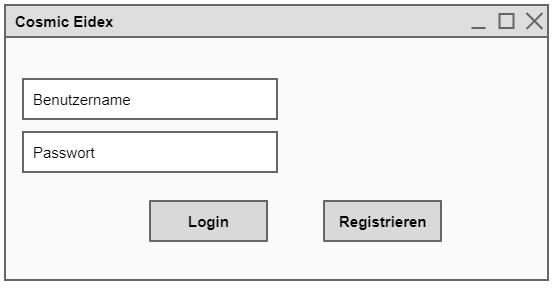
\includegraphics[width = 0.9\textwidth]{SEP_Lasten_Pflichtenheft/img/login_screen.png}
	\caption{Login-Seite}
	\label{gui:login}
\end{figure}

\begin{figure}[!h]
	\centering
	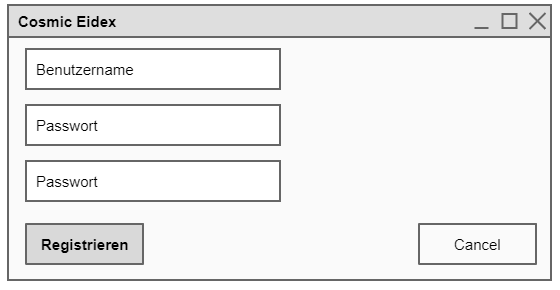
\includegraphics[width = 0.9\textwidth]{SEP_Lasten_Pflichtenheft/img/Registration Screen.png}
	\caption{Registration-Seite}
	\label{gui:registration}
\end{figure}

\begin{figure}[!h]
	\centering
	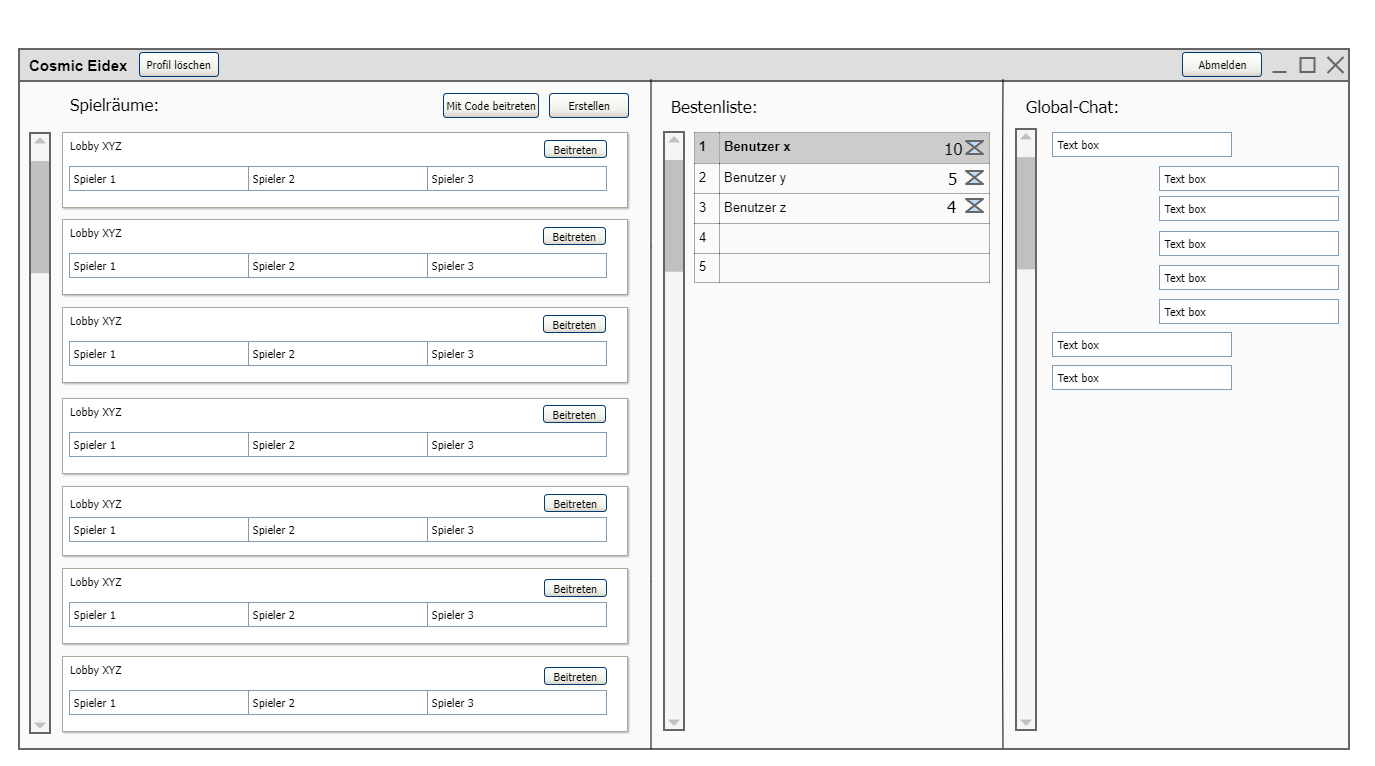
\includegraphics[width = 0.9\textwidth]{SEP_Lasten_Pflichtenheft/img/Looby Screen.png}
	\caption{Lobby-Seite}
	\label{gui:lobby}
\end{figure}

\begin{figure}[!h]
	\centering
	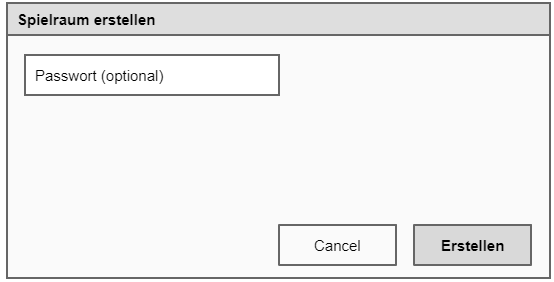
\includegraphics[width = 0.9\textwidth]{SEP_Lasten_Pflichtenheft/img/erstellen.png}
	\caption{Spielraum-Erstellungs-Seite}
	\label{gui:create_gameroom}
\end{figure}

\begin{figure}[!h]
	\centering
	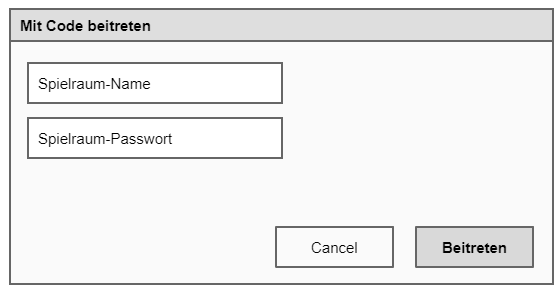
\includegraphics[width = 0.9\textwidth]{SEP_Lasten_Pflichtenheft/img/Mit Code Beitreten.png}
	\caption{Spielraumbeitritt per Code Seite}
	\label{gui:join_code}
\end{figure}

\begin{figure}[!h]
	\centering
	\includegraphics[width = 0.9\textwidth]{SEP_Lasten_Pflichtenheft/img/Profil löschen screen.png}
	\caption{Profil löschen Seite}
	\label{gui:delete_prof}
\end{figure}

\begin{figure}[!h]
	\centering
	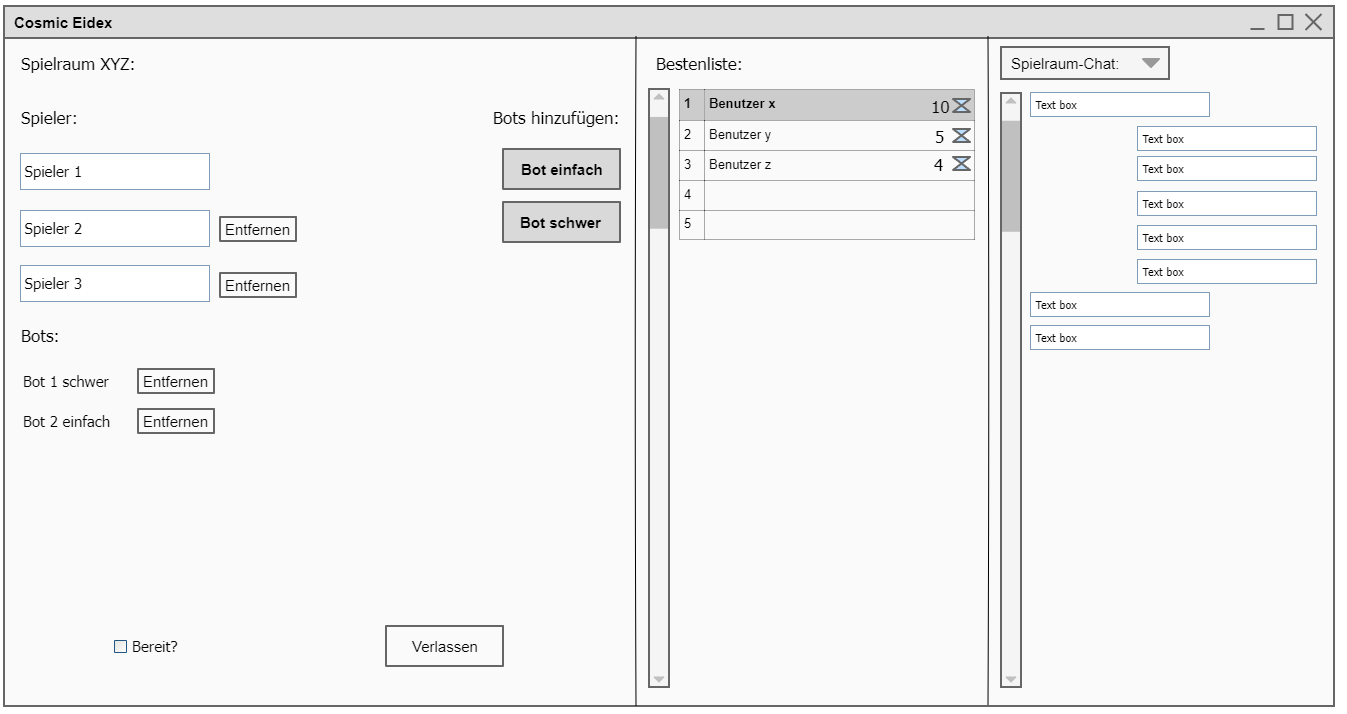
\includegraphics[width = 0.9\textwidth]{SEP_Lasten_Pflichtenheft/img/Spielraum-Screen.png}
	\caption{Spielraum-Seite}
	\label{gui:gameroom}
\end{figure}

\begin{figure}[!h]
	\centering
	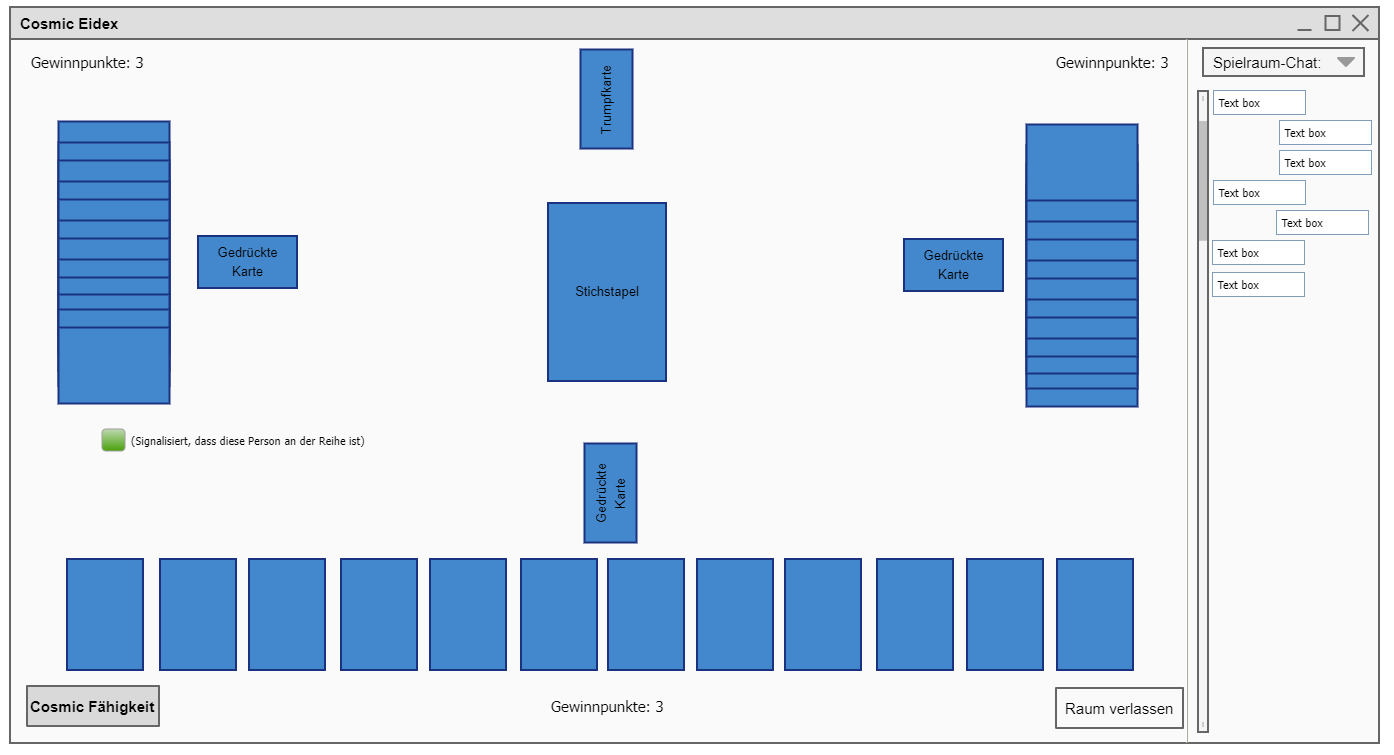
\includegraphics[width = 0.9\textwidth]{SEP_Lasten_Pflichtenheft/img/game_board_screen.png}
	\caption{Spielbrett-Seite}
	\label{gui:gameboard}
\end{figure}

\begin{figure}[!h]
	\centering
	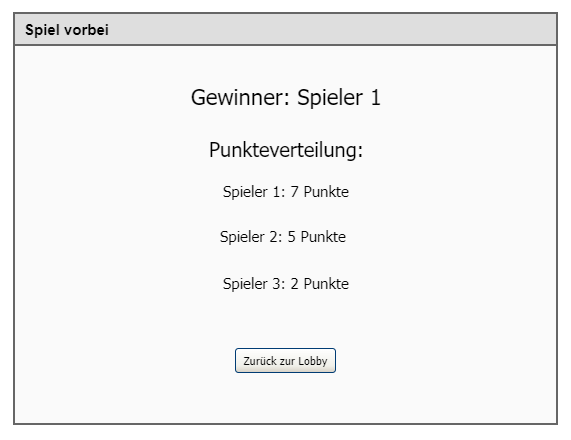
\includegraphics[width = 0.9\textwidth]{SEP_Lasten_Pflichtenheft/img/win_screen.png}
	\caption{Spielende-Seite}
	\label{gui:win}
\end{figure}	
	\chapter{Systemtestfälle}

\newcounter{tf}\setcounter{tf}{10}

\begin{description}[leftmargin=5em, style=sameline]

\begin{lhp}{tf}{TF}{tests:anmelden}
	\item [Name:] Spieler anmelden.
	\item [Motivation:] Testet, ob die Anmeldung in das System korrekt funktioniert.
	\item [Szenarien:] \hfill
		\begin{enumerate}
			\item \textit{Zugriffsdaten sind vorhanden und richtig} \\ $\implies$ Spieler wird in die Lobby bewegt.
			\item \textit{Benutzername ist registriert, Passwort ist falsch} \\ $\implies$ Fehlermeldung wird angezeigt.
			\item \textit{Benutzername ist nicht registriert} \\ $\implies$ Fehlermeldung wird angezeigt.
		\end{enumerate}
	\item [Relevante Systemfunktionen:] \ref{funk:zugriff}
	\item [Relevante Use Cases:] \ref{uc:anmeld}
\end{lhp}
\begin{lhp}{tf}{TF}{tests:löschen}
	\item [Name:] Spieler löschen
	\item [Motivation:] Testet, ob die authentifizierte 
          Spieler selbst  sein Konto löschen kann.
	\item [Szenarien:] \hfill
		\begin{enumerate}
			\item \textit{Spieler ist eingeloggt und bestätigt die Löschung mit korrektem Passwort} \\ $\implies$ Konto wird gelöscht, Spieler wird ausgeloggt und zur Startseite weitergeleitet.
			\item \textit{ Spieler ist eingeloggt, gibt aber ein falsches Passwort zur Bestätigung ein} \\ $\implies$ Fehlermeldung wird angezeigt, Konto bleibt bestehen.
			\item \textit{Spieler ist nicht eingeloggt und ruft die „Konto löschen“-Funktion auf} \\ $\implies$ Fehlermeldung oder Weiterleitung zum Login.
            \item \textit{Spieler erhält eine Bestätigungs-E-Mail über die erfolgreiche Löschung.} \\ $\implies$ E-Mail wird korrekt versendet, enthält Informationen zur Datenlöschung.
		\end{enumerate}
	\item [Relevante Systemfunktionen:] \ref{funk:zugriff}
	\item [Relevante Use Cases:] \ref{uc:löschen}
\end{lhp}
\begin{lhp}{tf}{TF}{tests:hinzufügen}
	\item [Name:] Spieler zum Spielraum hinzufügen
	\item [Motivation:] Testen, ob das Hinzufügen eines Spielers in einem Spielraum erfolgreich ist. 
	\item [Szenarien:] \hfill
		\begin{enumerate}
        \item \textit{Raum hat freien Platz} \\ $\implies$ Spieler kann im Raum hinzugefügt werden.
            \item \textit{Der Raum ist voll} \\ $\implies$  Fehlermeldung wird angezeigt.
		\end{enumerate}
	\item [Relevante Systemfunktionen:] \ref{funk:spielraum}
	\item [Relevante Use Cases:] \ref{uc:spielerlobbyhinzufuegen}
\end{lhp}
\begin{lhp}{tf}{TF}{tests:bot}
	\item [Name:] Bot hinzufügen
	\item [Motivation:] Testen, ob Bots in Spielräumen hinzugefügt wurden. 
	\item [Szenarien:] \hfill
		\begin{enumerate}
        \item \textit{Raum hat freien Platz} \\ $\implies$ Bot wird im Raum hinzugefügt.
            \item \textit{Der Raum ist voll} \\ $\implies$  Fehlermeldung wird angezeigt.
            \item \textit{Der Spieler, der den Bot hinzufügen möchte, ist nicht der Host} \\ $\implies$  Fehlermeldung wird angezeigt.
		\end{enumerate}
	\item [Relevante Systemfunktionen:] \ref{funk:bots}
	\item [Relevante Use Cases:] \ref{uc:botersetzen}
\end{lhp}
\begin{lhp}{tf}{TF}{tests:bot}
	\item [Name:]Starten eines Spiels.
	\item [Motivation:] Testen, ob ein Spiel gestartet werden kann. 
	\item [Szenarien:] \hfill
		\begin{enumerate}
        \item \textit{Es gibt eine ausreichende Anzahl von Spielern im Spielraum} \\ $\implies$ Das Spiel wurde erfolgreich gestartet
            \item \textit{Die Anzahl der Spieler im Spielraum ist nicht ausreichend} \\ $\implies$  Das Spiel startet nicht.
		\end{enumerate}
	\item [Relevante Systemfunktionen:] \ref{funk:spielverw}
	\item [Relevante Use Cases:] \ref{uc:spielbeginnen}
\end{lhp}
\begin{lhp}{tf}{TF}{tests:ausfuehren}
	\item [Name:] Spielzug ausgeführt.
	\item [Motivation:] Testen, ob ein Spielzug gut ausgeführt wird 
	\item [Szenarien:] \hfill
		\begin{enumerate}
        \item \textit{Der Spieler führt einen Zug aus, der mit den Regeln übereinstimmt} \\ $\implies$ Der nächste Spieler ist nun am Zug
            \item \textit{Der Spieler macht einen Zug, der nicht mit den Regeln übereinstimmt} \\ $\implies$  Fehlermeldung wird angezeigt.
            \end{enumerate}
	\item [Relevante Systemfunktionen:] \ref{funk:spielverw}
	\item [Relevante Use Cases:] \ref{uc:spielzugausfuehren}
\end{lhp}
\begin{lhp}{tf}{TF}{tests:aktualisieren}
	\item [Name:]Bestenliste.
	\item [Motivation:] Testen, ob die Bestenliste den Punktestand anzeigt und auch nach dem Ende eines Spiels aktualisiert wird.
	\item [Szenarien:] \hfill
		\begin{enumerate}
        \item \textit{Das Spiel ist vorbei} \\ $\implies$ Die Bestenliste aktualisiert den Punktestand.
            \item \textit{Es wurde noch kein Spiel gespielt} \\ $\implies$  Meldung wird angezeigt.
		\end{enumerate}
	\item [Relevante Systemfunktionen:] \ref{funk:bestenliste}
	\item [Relevante Use Cases:] \ref{uc:bestenlisteanzeigen}
\end{lhp}
\begin{lhp}{tf}{TF}{tests:aktualisieren}
	\item [Name:]Schreiben im Chat.
	\item [Motivation:] Testen, ob ein Spieler eine Nachricht im Chat senden kann.  
	\item [Szenarien:] \hfill
		\begin{enumerate}
        \item \textit{Der Spieler sendet eine Nachricht} \\ $\implies$ Die Nachricht wird von anderen Spielern gesehen.
		\end{enumerate}
	\item [Relevante Systemfunktionen:] \ref{funk:chat}
	\item [Relevante Use Cases:] \ref{uc:chatnachricht}
\end{lhp}
\end{description}
	\chapter{Warteraum}

Hier werden Anforderungen spezifiziert die den sogenannten ``Warteraum'' darstellen. Hier gehören alle Anforderungen, die ``Wünschkriterien'' sind, das heißt, sie sind zwar erwünscht, aber werden nur dann in aktuelle Anforderungen übernommen, wenn dafür genügendes Zeitbudget vorhanden ist und werden am wahrscheinlichsten in der Zukunft (und nicht jetzt) implementiert (oder in den kommenden Sprints beim SCRUM-Prozessmodell).

\newcounter{wr}\setcounter{wr}{10}

\begin{description}[leftmargin=5em, style=sameline]	
	\begin{lhp}{wr}{WR}{nfunk:sarch1}
		\item [Name:] Hintergrundmusik
		\item [Beschreibung:] Für die Spieler soll eine Auswahl zur Verfügung stehen, mit der die Hintergrundmusik beim Spielen ausgewählt werden kann.
		\item [Motivation:] Höhere Zufriedenheit der Benutzer.
		\item [Erfüllungskriterium:] Spieler können zu jedem Zeitpunkt (außer im Vorraum) die Musik ausschalten oder ein anderes Lied auswählen.
	\end{lhp}
\end{description}
	
\end{document}
